\documentclass{article}

% NeurIPS 2025 camera-ready style, non-anonymous (course individual report).
\usepackage[preprint]{neurips_2025}

\usepackage[utf8]{inputenc}
\usepackage[T1]{fontenc}
\usepackage{amsmath,amssymb,amsthm}
\usepackage{booktabs}
\usepackage{graphicx}
\usepackage{hyperref}

\graphicspath{{../figures/}}

% The report has several floats; tighten the spacing around them.
\setlength{\textfloatsep}{5pt plus 2pt minus 2pt}
\setlength{\floatsep}{5pt plus 2pt minus 2pt}
\setlength{\intextsep}{5pt plus 2pt minus 2pt}
\setlength{\abovecaptionskip}{3pt}
\setlength{\belowcaptionskip}{0pt}
\setlength{\parskip}{0pt}

% allow float-dense pages: the default fractions leave large gaps of white space
\renewcommand{\topfraction}{0.94}
\renewcommand{\bottomfraction}{0.80}
\renewcommand{\textfraction}{0.05}
\renewcommand{\floatpagefraction}{0.70}
\setcounter{topnumber}{4}
\setcounter{totalnumber}{8}

\newtheorem{lemma}{Lemma}
\newtheorem{proposition}{Proposition}

\newcommand{\R}{\mathbb{R}}
\newcommand{\Proj}{\operatorname{Proj}}
\newcommand{\eFeas}{e_{\mathrm{feas}}}
\newcommand{\eObj}{e_{\mathrm{obj}}}
\newcommand{\Tol}[1]{10^{-#1}}

\title{ADMM and Primal--Dual Hybrid Gradient for Discrete Optimal Transport:\\ A Comparative Study of a Constrained Linear Program}

\author{%
  Yu Kaijing \\
  Student ID: 25145003r \\
  \texttt{COMP 6704 Advanced Topics in Optimization} \\
  The Hong Kong Polytechnic University
}

\begin{document}

\maketitle

\begin{abstract}
Discrete optimal transport (OT) is a linear program with two families of marginal
equality constraints and a non-negativity constraint. We implement from scratch two
first-order methods for it: ADMM, applied to the affine marginal set through a
closed-form Euclidean projection, and PDHG of Chambolle and Pock on the saddle-point
form, together with three enhancements from the first-order LP literature (residual
balancing of the ADMM penalty, adaptive restarting of PDHG, and diagonal
preconditioning). Both are benchmarked against HiGHS dual simplex, used only as a
high-accuracy reference, on 40 synthetic instances
($m=n\in\{20,50,100,200\}$, uniform and nonuniform marginals) and 20 handwritten-digit
problems, under one budget, with feasibility and objective errors measured separately.
An entropically regularised (Sinkhorn) solver runs as a fourth baseline on the same
unregularised metrics, and every run carries a dual-gap certificate that bounds its
suboptimality without the reference value.

The objective error crosses the tolerance well before the feasibility error, so the marginal
constraint, not the objective, limits an accurate solution. Marginal shape matters more than
problem size: at $m=n=200$ the residual is up to ten orders larger on nonuniform marginals,
and eight times the budget recovers about one, so the gap is budget-limited rather than
intrinsic. With its penalty tuned on disjoint pilots ADMM solves everything at both
tolerances while PDHG fails on half of the largest, and none of the three enhancements helps.
The certificate certifies $130$ of the $160$ runs at $\Tol{4}$ without a reference value, and
shows the Sinkhorn bias is set by $\varepsilon$ rather than intrinsic: pushing $\varepsilon$
two orders below the grid meets the two-sided tolerance on $38$ of $40$ instances, at about
three times the cost.\footnote{Source, raw results, figures and a one-command
reproduction script: \url{https://github.com/kaijingyu41-ctrl/COMP6704}.}
\end{abstract}

\section{Introduction}

Given a supply distribution $a$ over $m$ locations, a demand distribution $b$ over
$n$ locations, and a cost $C_{ij}$ of moving one unit of mass from $i$ to $j$,
discrete optimal transport asks for the cheapest way of moving all the mass:
\begin{equation}
\label{eq:ot}
\min_{X\in\R^{m\times n}}\ \langle C,X\rangle
\quad\text{s.t.}\quad
X\mathbf 1_n=a,\qquad X^\top\mathbf 1_m=b,\qquad X\ge 0 .
\end{equation}
This is the Kantorovich formulation \citep{kantorovich1942}, a linear program whose
difficulty comes from its constraints: two families of marginal equalities plus
elementwise non-negativity. It underlies image retrieval, colour transfer, domain
adaptation and generative modelling \citep{peyre2019}, and it is hard to solve to high
accuracy with first-order methods. The feasible set is a transportation polytope in $mn$
variables, projecting onto it is not free, and the methods that do reach machine
precision need factorisations that scale poorly.

\paragraph{Scope.}
The group presentation of this course covers unconstrained optimisation; this project studies
the opposite regime, where every algorithm handles constraints and restores the marginals or
the non-negativity constraint exactly at each iteration.

\paragraph{Contributions.}
We derive the closed-form Euclidean projection onto the affine marginal set
(Lemma~\ref{lem:projection}) and implement from scratch an ADMM splitting, with the
marginals in one block and non-negativity in the other, and PDHG on the saddle-point
form; both use $O(mn)$ time per iteration and never form the constraint matrix. We also
implement and evaluate residual balancing, adaptive restarting and diagonal
preconditioning. The dual-gap certificate of Proposition~\ref{prop:certificate} bounds
the suboptimality of any non-negative iterate from the potentials the solvers already
maintain, so optimality can be judged without a reference solve, and we reuse those
potentials to audit the reference itself. Finally we build a controlled benchmark of 40
synthetic and 20 real instances that separates feasibility from optimality. The
splittings, the enhancements and the regularised baseline come from the cited work and
are used as published; the gap is the classical primal--dual gap, and what is specific
here is reading it off the solvers' own potentials, requiring feasibility alongside it,
and reusing it to audit the reference.

\section{Related work}

\paragraph{Optimal transport.}
The theory is in \citet{villani2009} and the computational side in \citet{peyre2019}.
Entropic regularisation makes the problem solvable by Sinkhorn iterations
\citep{cuturi2013}, and \citet{benamou2015} iterate closed-form Bregman projections onto
the constraint sets of the regularised problem, which is a different projection from our
Euclidean one. The regularisation bias is of order $\varepsilon\log(mn)$
\citep{peyre2019}, so Sinkhorn is kept only as a baseline measured on the unregularised
metrics (Section~\ref{sec:sinkhorn}). First-order LP codes judge a point by a computable
duality gap rather than against a solved instance \citep{applegate2021pdlp}; that is the
alternative to a reference solver used in Proposition~\ref{prop:certificate}.

\paragraph{Splitting methods.}
ADMM \citep{boyd2011admm} is the Douglas--Rachford splitting \citep{eckstein1992}
applied to the dual, with an $O(1/k)$ rate on two-block convex problems
\citep{he2012rate}. Its behaviour depends strongly on the penalty $\rho$, which motivated
the residual-balancing rule \citep{he2012rate} and the adaptive schemes of
\citet{goldstein2014} tested in Section~\ref{sec:sensitivity}. That rate holds
unconditionally here, since a linear objective is not strongly convex, the assumption
behind the linear rates of \citet{deng2016linear}; LP-type problems can still converge
linearly through a global error bound \citep{yang2016linear}, and a badly scaled marginal
distribution is where that constant suffers. PDHG \citep{chambolle2011} underlies the
state of the art in first-order LP: PDLP \citep{applegate2021pdlp,applegate2025pdlp} adds
preconditioning, adaptive steps, restarting, presolving and polishing and solves
instances with billions of non-zeros, while ours is the plain version. The reference is
HiGHS dual simplex \citep{huangfu2018highs}, called through SciPy.

\section{Problem formulation}
\label{sec:formulation}

Let $a\in\R^m$ and $b\in\R^n$ with $a,b\ge0$ and $\sum_i a_i=\sum_j b_j=1$. The balance
condition is necessary for \eqref{eq:ot} to be feasible, and under it $X=ab^\top$
satisfies all three constraints. Since $X\mathbf 1=a$ together with $X\ge0$ forces
$0\le X_{ij}\le a_i\le1$, the feasible set is a non-empty compact subset of
$[0,1]^{m\times n}$ and an optimum is attained.

The Lagrangian dual of \eqref{eq:ot} is
\begin{equation}
\label{eq:dual}
\max_{\alpha\in\R^m,\ \beta\in\R^n}\ \ a^\top\alpha+b^\top\beta
\qquad\text{s.t.}\qquad
\alpha_i+\beta_j\le C_{ij}\ \ \forall i,j ,
\end{equation}
and LP duality equates the two optimal values. A primal feasible $X$ and a dual feasible
$(\alpha,\beta)$ are both optimal exactly when complementary slackness holds,
\begin{equation}
\label{eq:cs}
X_{ij}\bigl(C_{ij}-\alpha_i-\beta_j\bigr)=0 \qquad \forall i,j .
\end{equation}
We use \eqref{eq:cs} only as a unit-test certificate. The benchmark uses the reference
objective value, so no method receives information its competitors lack.

\paragraph{Two notions of accuracy.}
Reporting only $\langle C,X\rangle$ is not sufficient. Scaling down a negative entry
lowers the objective without producing a valid plan, so a low objective can be bought by
giving up feasibility. We therefore report
\begin{equation}
\eFeas(X)=\|X\mathbf 1_n-a\|_1+\|X^\top\mathbf1_m-b\|_1,
\qquad
\eObj(X)=\bigl|\langle C,X\rangle-f_{\mathrm{ref}}\bigr| ,
\end{equation}
and call a run \emph{solved at tolerance $\varepsilon$} only when both errors are
$\le\varepsilon$ at some logged iterate. Each method returns its last iterate, so a run
counted as solved can return a slightly worse plan, the worst case being
$\eFeas=1.6\times\Tol{4}$. Non-negativity holds by construction in every method. Two
caveats apply: $f_{\mathrm{ref}}$ is a double-precision value rather than a symbolic
optimum, so objective differences are not evidence below the accuracy of the reference,
which Section~\ref{sec:certificate} audits instead of assuming; and the optimal plan need
not be unique, so two correct solvers may return different matrices.

\paragraph{An optimality certificate that needs no reference solution.}
The objective error above presumes that a high-accuracy solve has already been paid for.
The quantities we must report anyway contain a classical alternative.

\begin{proposition}[Dual-gap certificate]
\label{prop:certificate}
Let $T\ge0$ and let $(\alpha,\beta)$ satisfy $\alpha_i+\beta_j\le C_{ij}$ for all
$i,j$. Then
\begin{equation}
\label{eq:certificate}
\langle C,T\rangle-f^\star
\;\le\;
\underbrace{\bigl\langle C-\alpha\mathbf 1^\top-\mathbf 1\beta^\top,\,T\bigr\rangle}_{\text{complementarity defect}}
+\underbrace{\alpha^\top(T\mathbf 1_n-a)+\beta^\top(T^\top\mathbf 1_m-b)}_{\text{marginal violations, priced}},
\end{equation}
and the right-hand side is computable from $T$ alone.
\end{proposition}
\begin{proof}
Adding and subtracting $a^\top\alpha+b^\top\beta$ from $\langle C,T\rangle$ gives
\[\langle C,T\rangle-(a^\top\alpha+b^\top\beta)
=\langle C-\alpha\mathbf 1^\top-\mathbf 1\beta^\top,T\rangle
+\alpha^\top(T\mathbf 1_n-a)+\beta^\top(T^\top\mathbf 1_m-b),\]
using $\langle\alpha\mathbf 1^\top,T\rangle=\alpha^\top T\mathbf 1_n$ and
$\langle\mathbf 1\beta^\top,T\rangle=\beta^\top T^\top\mathbf 1_m$. The right-hand
side is the bound in \eqref{eq:certificate}. Since $(\alpha,\beta)$ is dual feasible,
weak duality gives $a^\top\alpha+b^\top\beta\le f^\star$, and subtracting
$a^\top\alpha+b^\top\beta$ from both sides of $\langle C,T\rangle$ can only increase
the left-hand side. \end{proof}

The bound holds for any non-negative $T$ and any dual feasible pair, and its right-hand
side equals the primal--dual gap $\langle C,T\rangle-(a^\top\alpha+b^\top\beta)$. For a
primal feasible $T$ the gap therefore vanishes only when both members are optimal, and one
optimal side is not enough: with $C\equiv1$ on a $2\times2$ problem with uniform marginals
every feasible plan is optimal, so $\langle C,T\rangle=f^\star=1$, yet $\alpha=\beta=0$
gives a bound of $1$. The last two terms price marginal violations, so a small bound does
not certify an infeasible plan either: with $T=0$ and $\alpha=\beta=0$ it is zero although
$T$ is not a plan. Being an upper bound, it never shows that the error is large.

Both methods already carry the ingredients. ADMM's projected block satisfies
$C+\rho(X-Z+U)=\alpha\mathbf 1^\top+\mathbf 1\beta^\top$ exactly, so the potentials can be
read off the stationarity residual of the $X$ block, provided it is formed with the $Z,U$
used inside the projection, since the update would otherwise destroy its additively
separable form; PDHG carries the multiplier of the marginal equalities as its dual
iterate. Neither pair is feasible in general, so we repair it with
$\beta_j\leftarrow\min_i(C_{ij}-\alpha_i)$, the largest value that makes the pair feasible
for the given $\alpha$. A candidate that was already feasible can only see $\beta$ grow,
so the bound tightens; one that was not has $\beta$ cut back and the bound loosens.

\paragraph{The affine projection has a closed form.}
Non-negativity is trivial to enforce, but re-imposing the marginals is not; the next
lemma shows the marginals alone are easy, because they define an affine set.

\begin{lemma}[Euclidean projection onto the marginal set]
\label{lem:projection}
Let $\mathcal A=\{X\in\R^{m\times n}: X\mathbf 1_n=a,\ X^\top\mathbf 1_m=b\}$ with
$\sum_i a_i=\sum_j b_j=1$. Then for any $W$,
\begin{equation}
\label{eq:proj}
\bigl[\Proj_{\mathcal A}(W)\bigr]_{ij}
=W_{ij}+\frac{r_i}{n}+\frac{s_j}{m}-\frac{d}{mn},
\quad
r=a-W\mathbf 1_n,\ \ s=b-W^\top\mathbf 1_m,\ \ d=1-\textstyle\sum_{ij}W_{ij}.
\end{equation}
\end{lemma}
\begin{proof}
Write $P$ for the right-hand side of \eqref{eq:proj}. Summing $P$ over $j$ and
using $\sum_j s_j=d$ gives
$(P\mathbf 1_n)_i=W\mathbf 1_{n,i}+r_i+\tfrac{d}{m}-\tfrac{d}{m}=W\mathbf 1_{n,i}+r_i=a_i$,
and summing over $i$ gives $(P^\top\mathbf 1_m)_j=W^\top\mathbf 1_{m,j}+s_j=b_j$, so
$P\in\mathcal A$. For optimality, let $D$ satisfy $D\mathbf 1_n=0$ and
$D^\top\mathbf 1_m=0$. Every term of $W-P$ carries a factor $u\mathbf 1^\top$,
$\mathbf 1 v^\top$ or $\mathbf 1\mathbf 1^\top$, and
$\langle u\mathbf 1^\top,D\rangle=u^\top D\mathbf 1=0$,
$\langle \mathbf 1 v^\top,D\rangle=v^\top D^\top\mathbf 1=0$,
$\langle \mathbf 1\mathbf 1^\top,D\rangle=\mathbf 1^\top D\mathbf 1=0$, so
$\langle W-P,D\rangle=0$. Every $X\in\mathcal A$ differs from $P$ by such a $D$, hence
$\langle W-P,X-P\rangle=0$ for all $X\in\mathcal A$. Since $\mathcal A$ is an affine
subspace containing $P$, that is the first-order condition for the projection, and the
projection is unique.
\end{proof}

Equation~\eqref{eq:proj} costs two row/column summations and two outer products, so
$O(mn)$ time and no factorisation. It does not enforce non-negativity, which is why a
second block is needed.

\paragraph{Cost model.}
Costs are rescaled affinely to $[0,1]$ and the marginals normalised to sum to one, which
leaves the optimal plans unchanged. All three solvers use $O(mn)$ time and memory per
iteration and never form the constraint matrix, so the comparison rests on the iteration
count. By the $O(1/k)$ \emph{ergodic} bound of \citet{he2012rate}, reaching a gap
$\varepsilon$ costs $O(mn/\varepsilon)$ work, against $O(\log(1/\varepsilon))$ for the
linear rate of \citet{yang2016linear} under a favourable error-bound constant. Simplex
and interior-point methods reach machine precision but need faster-growing factorisations
\citep{applegate2021pdlp}. We do not fit a scaling exponent, since four sizes cannot
support one.

\section{Methods}
\label{sec:methods}

\subsection{ADMM with an exact affine projection}
\label{sec:admm}

We split the two constraint families by introducing a copy $Z$,
\begin{equation}
\label{eq:splitting}
\min_{X,Z\in\R^{m\times n}}\ \langle C,X\rangle+\mathcal I_{\mathcal A}(X)
+\mathcal I_{+}(Z)\qquad\text{s.t.}\qquad X=Z ,
\end{equation}
where $\mathcal I_{\mathcal S}$ is the indicator of $\mathcal S$. Both blocks are easy:
the proximal operator of $\mathcal I_{\mathcal A}$ is $\Proj_{\mathcal A}$, and that of
$\mathcal I_+$ is the elementwise positive part. With scaled dual $U$,
\begin{equation}
\label{eq:admm}
X^{k+1}=\Proj_{\mathcal A}\!\left(Z^k-U^k-\tfrac1\rho C\right),\quad
Z^{k+1}=\bigl(X^{k+1}+U^k\bigr)_+ ,\quad
U^{k+1}=U^k+X^{k+1}-Z^{k+1},
\end{equation}
initialised at $Z^0=ab^\top$, which is feasible, and $U^0=0$. Each block satisfies its
own constraint family exactly, so the algorithm moves the violation between the blocks
and shrinks it instead of trading it for a lower objective; neither block alone certifies
a solution, the pair does. We report $Z$, as do other ADMM formulations
\citep{boyd2011admm}.

\paragraph{Residual balancing.}
The classical remedy \citep{he2012rate,goldstein2014} compares the primal residual
$\|X^k-Z^k\|_F$ with the dual residual $\rho\|Z^k-Z^{k-1}\|_F$ and rescales $\rho$ to keep
them within a factor $\mu$, always rescaling $U$ by
$\rho_{\text{old}}/\rho_{\text{new}}$ so that the unscaled multiplier is unchanged. We
use $\mu=10$, $\tau=2$, check every $25$ iterations and stop adapting after $1000$.

\subsection{Primal--dual hybrid gradient}
\label{sec:pdhg}

Let $x=\mathrm{vec}(X)$, $c=\mathrm{vec}(C)$, $q=[a;b]$, and let
$Ax=[X\mathbf 1_n;\,X^\top\mathbf 1_m]$, so that $Ax-q$ stacks the two marginal
violations. Then \eqref{eq:ot} equals
$\min_{x\ge0}\max_y\langle c,x\rangle+\langle y,Ax-q\rangle$, and the Chambolle--Pock
scheme \citep{chambolle2011} gives
\begin{equation}
\label{eq:pdhg}
y^{k+1}=y^k+\sigma\bigl(A\bar x^k-q\bigr),\quad
x^{k+1}=\Bigl(x^k-\tau\bigl(c+A^\top y^{k+1}\bigr)\Bigr)_+ ,\quad
\bar x^{k+1}=2x^{k+1}-x^k .
\end{equation}
Convergence requires $\tau\sigma\|A\|_2^2<1$, and here $\|A\|_2^2=m+n$, attained at
$X=\mathbf 1\mathbf 1^\top/\sqrt{mn}$, so $\tau=\sigma=\eta/\sqrt{m+n}$ with $\eta<1$ is
safe and needs no tuning. Both operators are applied through reductions, and we
initialise $x^0=\mathrm{vec}(ab^\top)$, $\bar x^0=x^0$, $y^0=0$.

The two methods fail differently, which is what makes the comparison interesting. PDHG
keeps non-negativity exact at every iterate and only approaches the marginal equalities,
so it can return a non-negative matrix whose marginals are inaccurate; ADMM makes the
marginals exact in one block and non-negativity exact in the other, so the block we
report is non-negative and only approximately marginal-feasible, paired with an affine
block that is exactly marginal-feasible and may be negative.

\paragraph{Adaptive restart.}
PDLP \citep{applegate2021pdlp} restarts PDHG when a normalised duality gap fails to
decrease fast enough. We use a simpler test on the primal residual, which needs no
knowledge of the optimum: every $200$ iterations we compute $r^k=\|Ax^k-q\|_1$ and
compare it with the value $r^{k-200}$ recorded at the previous check; if
$r^k\ge(1-\beta)r^{k-200}$ we erase the extrapolation with $\bar x^k\leftarrow x^k$,
using $\beta=0.1$. The check and the update of its reference value happen at every
multiple of $200$ whether or not a restart fires, so the comparison is with the previous
check rather than the last restart, which is the PDLP variant we did not test; ignoring
the dual variable makes this weaker than PDLP's criterion.

\paragraph{Diagonal preconditioning.}
The Pock--Chambolle preconditioner replaces the scalar step sizes by
$\tau_j=1/\sum_i|A_{ij}|$ and $\sigma_i=1/\sum_j|A_{ij}|$. Every variable here appears in
exactly two constraints, so $\tau$ is the scalar $1/2$ and $\sigma_i$ equals $1/n$ on the
row constraints and $1/m$ on the column constraints. The condition
$\|\Sigma^{1/2}AT^{1/2}\|\le1$ is tight, so both steps are scaled by $\eta<1$;
Section~\ref{sec:sensitivity} reports that the variant does not help.

\subsection{Reference solver and evaluation protocol}

The reference is HiGHS dual simplex \citep{huangfu2018highs} through
\texttt{scipy.optimize.linprog}. The constraint matrix has rank $m+n-1$, its only linear
dependency being $\sum_i\text{row}_i=\sum_j\text{col}_j$, so we pass all $m$ row
constraints and the first $n-1$ column constraints; dropping two equations would enlarge
the feasible set and yield a wrong reference value. The returned plan is checked for
feasibility and the call rejected if the check fails.

Every first-order method gets the same budget, $5\times10^4$ iterations or $60$ seconds,
whichever comes first, with diagnostics every $25$ iterations. None stops early on a
residual test: such a test must require both residuals to be small, and the primal
residual alone can vanish spuriously, which on a degenerate $2\times2$ problem returned a
matrix whose absolute objective error was $0.4$ against a reference optimum of $0$.
Timing excludes data generation and plotting but includes all solver work, the
certificate, the dual repair and the polishing being applied after the clock is read. The
fixed-penalty ADMM uses $\rho$ frozen from the pilot study of
Section~\ref{sec:sensitivity}, whose seeds are disjoint from the evaluation grid (pilot
$10$--$15$, evaluation $0$--$4$). Each run also carries a certificate: the solver's
potentials are repaired into a dual feasible pair and fed to
Proposition~\ref{prop:certificate}. A run counts as \emph{certified} only when that bound
and the marginal error of the same plan are both below the tolerance, since the bound
alone can be small for an infeasible plan. The regularised baseline is a separate
experiment, because it solves a different problem.

\section{Experiments}
\label{sec:experiments}

\subsection{Setup}

\paragraph{Correctness instances.}
Three problems with known optima: a $2\times2$ diagonal-cost problem (optimum $0$,
unique plan $\mathrm{diag}(\tfrac12,\tfrac12)$); a $9\times7$ constant-cost problem
$C\equiv0.37$ (optimum $0.37$, all feasible plans optimal); and a $30\times30$ planted
permutation, $C_{ij}=0$ on the permutation and $1$ elsewhere (optimum $0$, unique plan
$n^{-1}P$).

\paragraph{Benchmarks.}
The synthetic grid uses $m=n\in\{20,50,100,200\}$, two marginal regimes and five seeds;
points are uniform in the unit square and the cost is the squared Euclidean distance
rescaled to $[0,1]$. The \emph{uniform-marginal} regime sets $a=b=\mathbf 1/n$; the
\emph{nonuniform} one draws $a$ and $b$ independently from Dirichlet$(0.2)$, producing
masses that span several orders of magnitude while keeping $\sum a=\sum b=1$. The
real-data benchmark uses twenty problems built from \texttt{load\_digits}
\citep{dua2017uci,pedregosa2011sklearn} (1797 grey-scale $8\times8$ images), ten with
matching labels and ten with different ones; an image's grey levels, normalised to sum to
one, form its marginal, the cost between two pixels is their squared Euclidean distance,
and pixels carrying less than $\Tol{6}$ of the mass are dropped, giving sparse supports of
$27$--$40$ points. All timings are single-process CPU-only Python 3.12 (NumPy 2.5, SciPy
1.18, scikit-learn 1.9, Matplotlib 3.11); HiGHS is compiled C++, so its time is context
rather than a like-for-like comparison.

\subsection{Correctness}

On the three analytically known instances every method reproduces the exact optimum to
machine precision and the planted permutation to within $1.6\times\Tol{14}$, and HiGHS
agrees with the analytic value in all three. The unit tests add four independent checks:
that \eqref{eq:proj} restores the marginals with a residual orthogonal to every feasible
direction, so it is the Euclidean projection; that $\langle Ax,y\rangle=\langle
x,A^\top y\rangle$; and that the plans returned by ADMM and PDHG satisfy the KKT conditions
of \eqref{eq:dual}--\eqref{eq:cs} against an independently solved dual. The tests assert
both errors, not only the objective.

\subsection{The objective converges before the marginals}
\label{sec:twosided}

Figure~\ref{fig:convergence} overlays the two error curves for three instances. In 22 of
the 24 (instance, method) traces the objective error crosses $\Tol{3}$ before the
feasibility error; the exceptions are the $10\times10$ and $20\times20$ uniform instances
under the fixed-penalty ADMM, where both cross within a few hundred iterations of each
other. Where it matters the effect is large. On the uniform $200\times200$ instance ADMM's
objective error reaches $\Tol{3}$ at iteration $50$ but its feasibility error only at
$2475$, and on the nonuniform instance the comparison is $225$ against $5025$; PDHG needs
$900$ against $4550$ and $2875$ against $22100$. A benchmark monitoring the objective
alone would stop tens of thousands of iterations too early, on iterates whose marginals
are wrong by up to $\Tol{2}$.

The mechanism is visible in the two ADMM blocks: the affine block $X$ satisfies the
marginals exactly but may be negative, so $\langle C,X\rangle$ can look excellent while
$X$ is not a plan, whereas the reported block $Z$ stays non-negative and only approaches
feasibility.

\begin{figure*}[t]
\centering
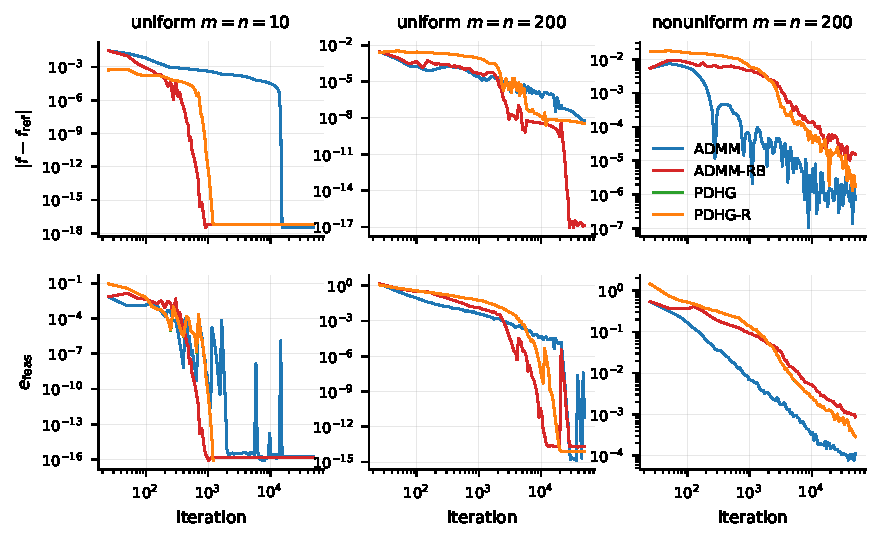
\includegraphics[width=0.46\textwidth]{fig2_convergence_iterations.pdf}
\caption{Objective error (top) and feasibility error (bottom) against the iteration
count for a uniform-marginal $10\times10$ instance, a uniform-marginal
$200\times200$ instance and a nonuniform $200\times200$ instance, all generated
with seed $0$. In every panel the objective curve crosses $10^{-3}$ before the
feasibility curve does.}
\label{fig:convergence}
\end{figure*}

\subsection{Scaling}

At $\Tol{3}$ every method solves every instance (Table~\ref{tab:main}), with median times
growing from $0.01$\,s at $m=n=20$ to $0.64$\,s for ADMM and $1.03$\,s for PDHG at $200$.
At $\Tol{4}$ the methods separate. The tuned ADMM solves every instance at every size,
with a median of $3.08$\,s at $m=n=200$, whereas PDHG is at $100\%$ for $m=n=20,50$,
$90\%$ at $100$ and $50\%$ at $200$, and residual-balancing ADMM at $90\%$, $50\%$ and
$50\%$ at the last three sizes. The failures are exactly the nonuniform-marginal
instances. Where PDHG does succeed its cheap iterations win, reaching $\Tol{4}$ on the
uniform $200\times200$ instance in $0.72$\,s against ADMM's $1.36$\,s, but it never does so
on the nonuniform instances that ADMM handles in $5.27$\,s.

\begin{table}[t]
\centering
\caption{Solve rate and median time in seconds to reach a tolerance, over $10$
instances per size (two marginal regimes, five seeds). A run counts as solved only
when both errors are below the tolerance; the time is the median over the runs that
reached it.}
\label{tab:main}
\small
\begin{tabular}{c}
\begin{tabular}{lcccc}
\toprule
Tolerance $10^{-3}$ & $m=n=20$ & $m=n=50$ & $m=n=100$ & $m=n=200$ \\
\midrule
ADMM & 100\% (0.01) & 100\% (0.03) & 100\% (0.10) & 100\% (0.64) \\
ADMM-RB & 100\% (0.01) & 100\% (0.05) & 100\% (0.44) & 100\% (3.94) \\
PDHG & 100\% (0.01) & 100\% (0.04) & 100\% (0.17) & 100\% (1.03) \\
PDHG-R & 100\% (0.01) & 100\% (0.04) & 100\% (0.17) & 100\% (1.03) \\
\bottomrule
\end{tabular}
\\[1.2ex]
\begin{tabular}{lcccc}
\toprule
Tolerance $10^{-4}$ & $m=n=20$ & $m=n=50$ & $m=n=100$ & $m=n=200$ \\
\midrule
ADMM & 100\% (0.02) & 100\% (0.07) & 100\% (0.35) & 100\% (3.08) \\
ADMM-RB & 100\% (0.02) & 90\% (0.03) & 50\% (0.08) & 50\% (0.77) \\
PDHG & 100\% (0.02) & 100\% (0.13) & 90\% (0.52) & 50\% (0.72) \\
PDHG-R & 100\% (0.02) & 100\% (0.13) & 90\% (0.50) & 50\% (0.71) \\
\bottomrule
\end{tabular}
\end{tabular}
\end{table}

\subsection{Marginal shape, more than problem size, limits the attainable accuracy}
\label{sec:mass}

Table~\ref{tab:mass} separates the two marginal regimes. Uniform-marginal instances are
essentially free: the tuned ADMM reaches $\Tol{3}$ in a median of $988$ iterations
($0.05$\,s) with a final feasibility error of $4.1\times\Tol{16}$, and PDHG's median final
feasibility error stays between $6.2\times\Tol{16}$ and $1.2\times\Tol{14}$. Nonuniform
instances cost the tuned ADMM only about $1.6$ times more iterations to reach $\Tol{3}$
($1562$ against $988$), but they settle far higher in error: its median final feasibility
error grows from $2.7\times\Tol{7}$ at $m=n=20$ to $5.3\times\Tol{5}$ at $200$, against
$6.8\times\Tol{12}$ in the uniform regime at that size, nearly seven orders apart. PDHG
separates further, ending at $2.1\times\Tol{4}$ on the nonuniform instances against
$1.2\times\Tol{14}$ on the uniform ones, a ten-order gap. At $\Tol{4}$ the uniform regime
is $100\%$ for every method, while on the nonuniform instances only the tuned ADMM still
reaches the tolerance, at $100\%$, against $70\%$ for PDHG and $45\%$ for residual
balancing.

Every instance is balanced transport in the standard sense; what differs is the \emph{shape}
of the marginals. The pattern points to a dynamic-range effect rather than a size effect:
under Dirichlet$(0.2)$ some marginal entries are of order $\Tol{5}$ or smaller while the cost
lies in $[0,1]$, so a method making uniform progress over all $mn$ variables must resolve
very large and very small masses at once.

\begin{table*}[t]
\centering
\caption{Effect of the marginal regime over all four sizes and five seeds. ``rate
(time)'' is the solve rate at $\Tol{3}$ and the median time of the solved runs;
``iters'' and $\eFeas$ are medians over all $20$ runs of the regime, including
those that did not reach the tolerance.}
\label{tab:mass}
\small
\begin{tabular}{lcccccc}
\toprule
Method & \multicolumn{3}{c}{Uniform} & \multicolumn{3}{c}{Dirichlet $\alpha=0.2$} \\
\cmidrule(lr){2-4}\cmidrule(lr){5-7}
 & rate (time) & iters & $e_{\mathrm{feas}}$ & rate (time) & iters & $e_{\mathrm{feas}}$ \\
\midrule
ADMM & 100\% (0.05) & 988 & $4.1{\times}10^{-16}$ & 100\% (0.07) & 1,562 & $1.1{\times}10^{-5}$ \\
ADMM-RB & 100\% (0.03) & 700 & $1.2{\times}10^{-14}$ & 100\% (0.46) & 10,125 & $1.3{\times}10^{-4}$ \\
PDHG & 100\% (0.04) & 1,438 & $2.4{\times}10^{-15}$ & 100\% (0.16) & 6,288 & $7.3{\times}10^{-5}$ \\
PDHG-R & 100\% (0.04) & 1,438 & $2.4{\times}10^{-15}$ & 100\% (0.16) & 6,288 & $7.3{\times}10^{-5}$ \\
\bottomrule
\end{tabular}
\end{table*}

\subsection{Certifying optimality without a reference solve}
\label{sec:certificate}

Every accuracy number so far is measured against $f_{\mathrm{ref}}$, so the tolerance
claims inherit its error. Proposition~\ref{prop:certificate} removes that dependence: each
solver already maintains dual potentials, and repairing them to dual feasibility turns
them into an upper bound on $\langle C,T\rangle-f^\star$ computed from the returned plan
alone. First-order LP codes use such a gap mainly to decide when to \emph{stop}
\citep{applegate2021pdlp}; we use it to decide whether the plan is correct and to audit the
reference itself. Table~\ref{tab:certificate} reports it beside the reference-based
objective error for every run of the main study.

The bound dominates the signed gap in all $160$ runs and is below $\Tol{4}$ in all $160$.
Neither fact certifies the plans by itself: the bound can be small because the plan is cheap
rather than optimal, and $30$ of the $160$ returned plans are not marginal-feasible at
$\Tol{4}$. The statement worth counting is the conjunction, which is what we mean by a
\emph{certified} run: the reported plan is feasible at the tolerance and its own bound is
below it. That holds for $130$ of the $160$ runs at $\Tol{4}$ and $159$ of $160$ at
$\Tol{3}$, and the $30$ failures are exactly the nonuniform instances identified in
Section~\ref{sec:mass}, so the certificate reproduces the main finding without any reference
value. Where the plans are accurate it is tight, with a median of $6.1\times\Tol{8}$ for the
tuned ADMM against a median reference-based error of $3.8\times\Tol{8}$, and on
uniform-marginal instances three of the four methods certify machine precision; it is looser
on the nonuniform ones, because marginal violations enter multiplied by dual prices of order
one. The bound is not a lower bound on the marginal residual, since the priced terms can
cancel and for PDHG the median bound on the nonuniform instances is negative, but it lives on
the same scale and in $60\%$ of the runs falls below the reference-based error.

\paragraph{An audit of the reference solver.}
Solving the dual LP independently and repairing it gives a dual feasible pair, so its
objective $L$ is a lower bound on $f^\star$ up to the rounding of that check; polishing the
reference plan gives a primal candidate whose objective $U$ is an upper bound on $f^\star$
provided the polishing reached feasibility, a condition the code checks and stores rather
than assumes. This is a numerical audit, not a certified interval; a rigorous one would have
to turn the residuals into corrections or use directed rounding. The interval is \emph{valid}
when that check passes and the endpoints agree to double precision, and the statistics filter
on that flag. Twenty-five of the $40$ synthetic instances and all $20$ digit instances
qualify, $f_{\mathrm{ref}}$ lies inside on all $45$, and the width there, which therefore
bounds the reference error from \emph{above}, is at most $2.9\times\Tol{9}$. On the other
$15$ the polish stalls and $U$ falls below $L$, leaving only $L\le f^\star$, a one-sided
statement: $|f_{\mathrm{ref}}-f^\star|\ge\max\{0,\,L-f_{\mathrm{ref}}\}$ on \emph{every}
instance. The positive part carries the information, being nonzero exactly where the
reference value sits below $L$; that happens on $14$ of the $40$ runs, by up to
$4.6\times\Tol{8}$, so the reference is in error by \emph{at least} that much. Its accuracy
is therefore \emph{not uniform}, a few $\Tol{9}$ on one half of the grid and no better than
$5\times\Tol{8}$ on the other, which is why objective differences here are not read as
evidence below about $\Tol{7}$.

\begin{table}[t]
\centering
\caption{Certified optimality bound against the reference-based objective error, medians
over the $10$ instances of each size. The bound uses no reference value; both panels
are on the same scale.}
\label{tab:certificate}
\footnotesize
\begin{tabular}{c}
\begin{tabular}{lcccc}
\toprule
certified bound & $m=n=20$ & $m=n=50$ & $m=n=100$ & $m=n=200$ \\
\midrule
ADMM & $9.8{\times}10^{-10}$ & $3.8{\times}10^{-8}$ & $4.5{\times}10^{-7}$ & $5.2{\times}10^{-7}$ \\
ADMM-RB & $5.7{\times}10^{-9}$ & $7.8{\times}10^{-17}$ & $5.3{\times}10^{-18}$ & $3.4{\times}10^{-18}$ \\
PDHG & $2.7{\times}10^{-18}$ & $-3.7{\times}10^{-18}$ & $1.6{\times}10^{-9}$ & $-9.9{\times}10^{-11}$ \\
PDHG-R & $3.6{\times}10^{-18}$ & $-5.3{\times}10^{-19}$ & $1.6{\times}10^{-9}$ & $-1.0{\times}10^{-10}$ \\
\bottomrule
\end{tabular}
\\[1.2ex]
\begin{tabular}{lcccc}
\toprule
error vs. reference & $m=n=20$ & $m=n=50$ & $m=n=100$ & $m=n=200$ \\
\midrule
ADMM & $3.3{\times}10^{-9}$ & $2.3{\times}10^{-8}$ & $6.3{\times}10^{-8}$ & $1.5{\times}10^{-7}$ \\
ADMM-RB & $5.7{\times}10^{-9}$ & $2.0{\times}10^{-7}$ & $1.9{\times}10^{-7}$ & $1.6{\times}10^{-7}$ \\
PDHG & $2.9{\times}10^{-8}$ & $1.6{\times}10^{-7}$ & $7.4{\times}10^{-8}$ & $2.9{\times}10^{-7}$ \\
PDHG-R & $2.9{\times}10^{-8}$ & $1.6{\times}10^{-7}$ & $7.6{\times}10^{-8}$ & $2.9{\times}10^{-7}$ \\
\bottomrule
\end{tabular}
\end{tabular}
\end{table}

\subsection{Is the residual a budget artefact?}
\label{sec:budget}

One budget leaves open whether a residual of $\Tol{4}$ is an intrinsic limit or simply
where the budget ran out. Running both methods eight times longer at the same settings and
reading the errors off the same trace at $50$k, $100$k, $200$k and $400$k iterations shows
that the residual keeps falling: on the two nonuniform $200\times200$ instances the ADMM
feasibility error drops from $1.1\times\Tol{4}$ and $7.7\times\Tol{5}$ to
$1.3\times\Tol{5}$ and $1.4\times\Tol{5}$, PDHG's from $2.8\times\Tol{4}$ and
$3.5\times\Tol{4}$ to $2.4\times\Tol{5}$ and $2.7\times\Tol{5}$, and the $100\times100$ instance decreases
monotonically at every checkpoint. The $50$k values reproduce the final errors of the main
study, so the gain is about one order of magnitude for eight times the budget, while the
uniform control, eight orders below the tolerance throughout, says nothing about the
nonuniform bottleneck. The $O(1/k)$ ergodic bound of \citet{he2012rate} predicts that trend
for the \emph{averaged} iterate, and we report the last one, so this is consistent with the
rate rather than a proof. It does establish that the methods have not stalled: the nonuniform
$\Tol{4}$ solve rates of Table~\ref{tab:mass} mean ``not reached within $5\times10^4$
iterations'' rather than ``unattainable''.

\subsection{The entropically regularised baseline}
\label{sec:sinkhorn}

Entropic regularisation is the standard way to solve a transport problem, so the question
is why the unregularised LP is solved here at all. Experiment G answers it on the seed-$0$
instances with the same budget, running a log-domain Sinkhorn iteration at
$\varepsilon\in\{0.2,0.1,0.05,0.02,0.01\}$ and handing the scaling vectors to the
certificate as the dual pair; they are the potentials of the marginal equalities, so they
need only be repaired to be tightened. A budget-matched ablation then pushes $\varepsilon$
two orders below that grid, with and without warm-started continuation, over the whole
grid.

The marginals are exact to machine precision at every $\varepsilon$ and size, worst case
$1.7\times\Tol{15}$, with no polishing, so what regularisation buys is feasibility rather
than accuracy. What it costs is optimality, and the cost is structural: the objective error
is proportional to $\varepsilon$ and does not decay with further iterations, because it is
the distance between two different problems. At $m=n=200$ the bias is $22$ times the optimum
on the uniform instance and $4.4$ times on the nonuniform one at $\varepsilon=0.2$. Measured
against the reference, the objective is above the stored reference value by at least
$1.3\times\Tol{3}$ in every one of the $40$ grid runs, and none of them meets the two-sided
$\Tol{4}$ criterion. The comparison runs in the safe direction: a reference that is too
\emph{low} inflates the bias rather than hiding it, and where the bracket on $f^\star$ closes
the reference error is at most $2.9\times\Tol{9}$, three orders below the smallest bias. The
certificate agrees, never falling below $3.9\times\Tol{3}$ over those runs, so not one of
them is certified at the tolerance; because the marginals are already exact, polishing
leaves it unchanged, so the certified gap is pure complementarity rather than a marginal
artefact. One sweep of the fixed budget costs $1.3$\,s at $m=n=20$ and $21.8$\,s at
$m=n=200$, about twice the tuned ADMM's full-budget cost at the largest size.

\paragraph{Does the grid simply stop too early?}
The obvious objection is that the grid never goes low enough, so
Table~\ref{tab:sinkhorncont} pushes $\varepsilon$ to $\Tol{4}$, two orders below the grid,
with warm-started continuation against a matched single-$\varepsilon$ control on the same
budget. The bias is controlled by $\varepsilon$ rather than intrinsic: at
$\varepsilon=\Tol{3}$ it is $1.2\times\Tol{4}$ and two runs in forty already meet the
two-sided criterion, at $\Tol{4}$ it falls to $1.7\times\Tol{6}$ and $38$ of $40$ do. A
regularised solver can therefore reach the LP tolerance, and the claim that none is certified
at $\Tol{4}$ holds only for $\varepsilon\ge0.01$. Continuation is what makes it affordable,
the same budget taking a median of $6.8$\,s against $15.9$\,s for a cold start, though at the
largest size the cold runs are cut off by the $60$\,s limit while the scheduled ones finish,
so this is a budget-and-time comparison rather than a like-for-like time-to-accuracy one. The
obstacle does move: at $\Tol{4}$ the median feasibility error is $3.3\times\Tol{6}$ against
$1.7\times\Tol{15}$ on the grid, because the plan concentrates on a vanishing fraction of the
$mn$ entries and the scaling vectors can no longer hold the marginals to machine precision.
What the unregularised formulation still buys is not reliability, since the tuned ADMM
certifies $39$ of the same $40$ instances at the same budget against $38$ and at about a
third of the wall-clock, but that the returned plan solves the stated problem rather than a
nearby one.

\begin{table}[t]
\centering
\caption{Does the regularised baseline improve if $\varepsilon$ is pushed two orders of
magnitude below the grid, and does warm-started continuation help? Both rows of each
pair were given the \emph{same} total iteration budget, so the comparison isolates the
schedule. Medians over the forty grid instances; ``certified@$\Tol{4}$'' is the
two-sided criterion of Section~\ref{sec:formulation}. The $\varepsilon$-sweep behind
the bias is in \texttt{tab\_sinkhorn.tex}.}
\label{tab:sinkhorncont}
\small
\begin{tabular}{lcccc}
\toprule
Variant & median $e_{\mathrm{obj}}$ & median bound & certified@$10^{-4}$ & time (s) \\
\midrule
single $\varepsilon=10^{-3}$ & $1.2{\times}10^{-4}$ & $3.9{\times}10^{-4}$ & 2/40 & 4.86 \\
schedule $\to 10^{-3}$ & $1.2{\times}10^{-4}$ & $3.9{\times}10^{-4}$ & 2/40 & 4.51 \\
single $\varepsilon=10^{-4}$ & $1.4{\times}10^{-6}$ & $2.1{\times}10^{-5}$ & 38/40 & 15.86 \\
schedule $\to 10^{-4}$ & $1.7{\times}10^{-6}$ & $2.1{\times}10^{-5}$ & 38/40 & 6.82 \\
\bottomrule
\end{tabular}
\end{table}

\subsection{Parameter sensitivity and ablations}
\label{sec:sensitivity}

Figure~\ref{fig:sensitivity} sweeps the ADMM penalty
$\rho\in\{0.1,1,10,100,1000\}$ and the PDHG step factor $\eta\in\{0.3,0.6,0.99\}$ on six
pilot instances whose seeds are disjoint from the evaluation seeds. The penalty matters a
great deal: $\rho=0.1$ reaches $\Tol{4}$ on two of the six instances, $\rho=1$ on three,
$\rho=10$ on five, and $\rho=100$ and $\rho=1000$ on all six, the worst-case final
feasibility error falling from $9.0\times\Tol{2}$ at $\rho=0.1$ to $1.4\times\Tol{5}$ at
$\rho=1000$. We adopt $\rho=100$ as the smallest value that solves every pilot instance;
$\rho=10$ would be faster on uniform marginals but fails one of the six. For PDHG the
median final feasibility error improves monotonically with $\eta$, from
$3.1\times\Tol{4}$ through $8.0\times\Tol{5}$ to $2.8\times\Tol{5}$ for $\eta=0.3,0.6,0.99$,
so $\eta\to1$ is both the largest step the theory allows and the best here.

None of the three enhancements improves on the plain method. \emph{Residual balancing}
keeps the $\Tol{3}$ solve rate but drops from $100\%$ to $67\%$ at $\Tol{4}$, its median
final feasibility error being $4.7\times\Tol{5}$ against $2.1\times\Tol{6}$, and it fails
eleven of the forty main-study instances where the fixed penalty fails none. The
\emph{restart} heuristic fires $107$--$241$ times per run on the evaluation grid, median
$186$, so its small effect is not because the criterion never triggers: it leaves the solve
rates and the median error unchanged and moves the final feasibility error of individual
instances by at most $2\%$. \emph{Diagonal preconditioning} is harmful, dropping the
$\Tol{3}$ solve rate to $83\%$ and the $\Tol{4}$ rate to $50\%$, with median final
feasibility error $1.0\times\Tol{4}$ against $2.8\times\Tol{5}$. One explanation is structural: a preconditioner built from $|A|$ is identical for every
instance, since $A$ has the same 0/1 sparsity pattern, so it cannot respond to the
data-dependent dynamic range of Section~\ref{sec:mass}; the data-dependent alternative,
rescaling the cost or the variables, is left untested. The steps also become unbalanced: at
$m=n=200$ the preconditioned primal step is $\eta/2\approx0.5$ against
$\eta/\sqrt{m+n}\approx0.05$.

\begin{figure}[t]
\centering
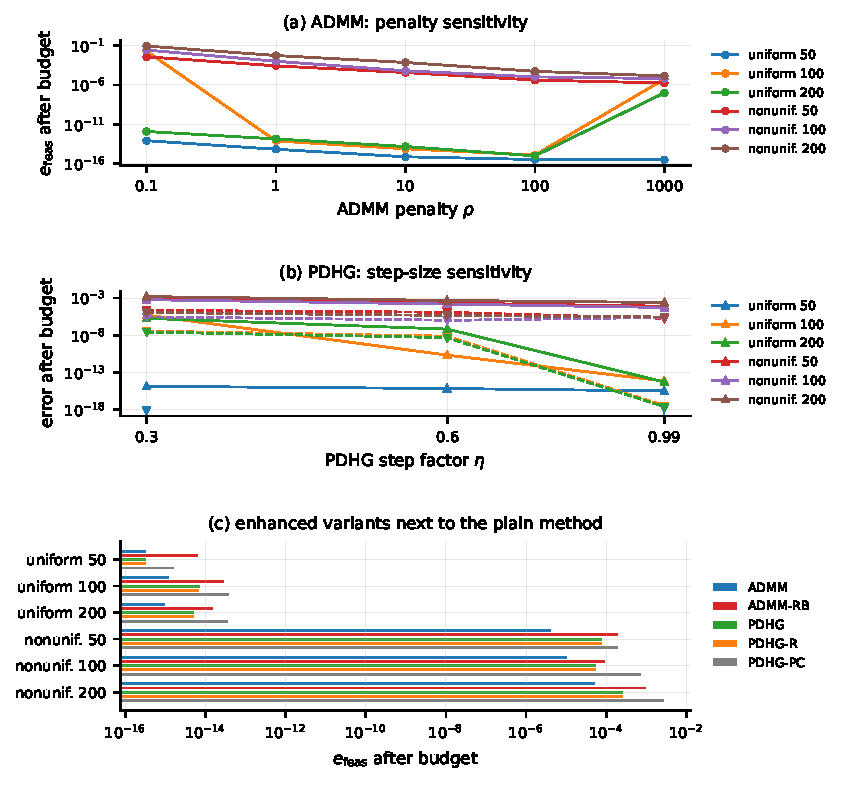
\includegraphics[width=0.40\textwidth]{fig7_parameter_sensitivity.pdf}
\caption{Parameter sensitivity and ablations of experiment C, on six pilot instances
($m=n\in\{50,100,200\}$ in each marginal regime, seeds $10$--$15$, uniform first).
(a) Final feasibility error after the budget against the ADMM penalty $\rho$, with the
ticks at the values actually tested. (b) The same against the PDHG step factor $\eta$
(solid), together with the objective error (dashed). (c) Final feasibility error of
each enhanced variant next to the plain method it is meant to improve, as horizontal
bars on a logarithmic axis.}
\label{fig:sensitivity}
\end{figure}

\subsection{Real handwritten-digit transport problems}

Table~\ref{tab:digits} reports the digit experiments. These problems are small, with
supports of $27$--$40$ points after thresholding, but structurally different from the
synthetic instances: the cost has low-rank structure because it is built from $8\times8$
grid geometry, and most mass entries are zero.

All four methods solve all twenty instances. ADMM is the most accurate at the budget, a
median feasibility error of $3.6\times\Tol{16}$ on same-label pairs and $3.9\times\Tol{16}$
on different-label pairs, with objective errors at machine epsilon and a worst case of
$6.0\times\Tol{16}$; it is also the fastest to the tolerance, $0.01$\,s median against
$0.02$\,s. PDHG is less uniform, $1.7\times\Tol{13}$ and $1.3\times\Tol{15}$ on same- and
different-label pairs, with a worst case of $1.3\times\Tol{9}$, more than six orders of
magnitude worse. This is the regime that most favours the two-block method, small sparse
problems where handling the marginals exactly pays off, and PDHG's tail here echoes its
failures on the largest synthetic instances. Same-label and different-label pairs behave
almost identically, since difficulty is governed by the support geometry and the marginal
dynamic range rather than by whether the two images depict the same digit. The couplings
concentrate mass between corresponding strokes.

\begin{table*}[t]
\centering
\caption{Handwritten-digit transport problems. ``rate (s)'' is the solve rate at
$\Tol{3}$ and the median time in seconds of the solved runs; $\eFeas$ and
$|f-f_{\mathrm{ref}}|$ are medians over all ten pairs of each kind.}
\label{tab:digits}
\small
\begin{tabular}{lcccccc}
\toprule
 & \multicolumn{3}{c}{same label} & \multicolumn{3}{c}{different label} \\
\cmidrule(lr){2-4}\cmidrule(lr){5-7}
Method & rate (s) & $e_{\mathrm{feas}}$ & $|f-f_{\mathrm{ref}}|$ & rate (s) & $e_{\mathrm{feas}}$ & $|f-f_{\mathrm{ref}}|$ \\
\midrule
ADMM & 100\% (0.01) & $3.6{\times}10^{-16}$ & $1.7{\times}10^{-18}$ & 100\% (0.01) & $3.9{\times}10^{-16}$ & $3.5{\times}10^{-18}$ \\
ADMM-RB & 100\% (0.02) & $7.4{\times}10^{-15}$ & $5.6{\times}10^{-17}$ & 100\% (0.02) & $8.7{\times}10^{-15}$ & $2.3{\times}10^{-16}$ \\
PDHG & 100\% (0.02) & $1.7{\times}10^{-13}$ & $4.9{\times}10^{-15}$ & 100\% (0.02) & $1.3{\times}10^{-15}$ & $2.2{\times}10^{-17}$ \\
PDHG-R & 100\% (0.02) & $1.6{\times}10^{-13}$ & $4.9{\times}10^{-15}$ & 100\% (0.02) & $1.3{\times}10^{-15}$ & $1.7{\times}10^{-17}$ \\
\bottomrule
\end{tabular}
\end{table*}

\subsection{Discussion and limitations}
\label{sec:discussion}

\paragraph{Which method to use.}
With the penalty tuned on disjoint pilot instances, ADMM is the better default here: it
solves every instance at both tolerances, including the nonuniform ones that PDHG fails on
half the time at $m=n=200$, and it is faster than PDHG at $\Tol{3}$ everywhere except the
smallest regime. PDHG keeps one advantage, its cheaper iterations winning at $\Tol{4}$ on
uniform-marginal instances, and it needs no tuning beyond the automatically safe
$\tau=\sigma=0.99/\sqrt{m+n}$. The caveat is that ADMM's superiority depends on tuning
$\rho$: with the untuned $\rho=10$ it fails one of the six pilot instances at $\Tol{4}$.

\paragraph{Limitations.}
The benchmark is CPU-only Python, so constant factors, and plausibly the comparison, would
change under a compiled or GPU implementation; five repeats move the timings by at most
$3.8\%$, so differences of a few percent are not significant. The Pock--Chambolle
preconditioner did not help (Section~\ref{sec:sensitivity}) and its data-dependent
alternative is untested. The largest instance has $m=n=200$, far from the regime where
first-order LP becomes indispensable, and four sizes are too few to fit a scaling exponent;
we evaluate the last iterate rather than the ergodic one. The reference audit is numerical
rather than a certified interval, so it fixes a scale, about $\Tol{7}$, below which objective
differences are not evidence. No method ranks uniformly across instances: on the five
$200\times200$ nonuniform instances the two ADMM variants differ by a factor of fifteen in
the median, $5.3\times\Tol{5}$ against $7.8\times\Tol{4}$, and the tuned ADMM's
uniform-marginal residual spans $1.3\times\Tol{15}$ to $5.5\times\Tol{6}$ across five seeds
of one family.

\section{Conclusion}
\label{sec:conclusion}

We implemented ADMM, whose affine block uses the closed-form projection of
Lemma~\ref{lem:projection} and keeps the marginals exact, and PDHG on the saddle-point form,
whose non-negativity is exact at every iterate while its marginal equalities are only
approached in the limit. Both were benchmarked against HiGHS on 40 synthetic and 20 real
instances under a criterion requiring feasibility and optimality together, each run carrying
a reference-free certificate alongside an entropically regularised baseline.

Marginal feasibility, not the objective, is the binding criterion: the objective error
crosses the tolerance first in almost every trace. Marginal shape rather than problem size
governs the attainable accuracy, ten orders of magnitude separating the regimes at
$m=n=200$, and eight times the budget recovers about one, so the difference lies in how fast
a budget buys accuracy rather than in a hard limit. With $\rho$ tuned on disjoint pilots ADMM
solves every instance at both tolerances while PDHG fails on half of the largest, and none of
the three enhancements helps. The certificate reproduces these findings without reference to
HiGHS, certifying $130$ of the $160$ runs at $\Tol{4}$, and audits the reference as well:
where its bracket closes the reference is pinned to $2.9\times\Tol{9}$, and elsewhere it lies
below a lower bound on $f^\star$ by up to $4.6\times\Tol{8}$. Entropic regularisation buys
exact marginals at the price of a gap no iterating removes at a \emph{fixed} $\varepsilon$,
and shrinking $\varepsilon$ buys it back on $38$ of $40$ instances at about three times the
cost.

% The reference list is set on its own page after the body.
\clearpage
\begin{thebibliography}{99}
\bibitem[Applegate et al.(2021)]{applegate2021pdlp}
D. Applegate et al. Practical large-scale linear programming using primal-dual
hybrid gradient. In \emph{NeurIPS}, 2021.

\bibitem[Applegate et al.(2025)]{applegate2025pdlp}
D. Applegate et al. PDLP: a practical first-order method for large-scale linear
programming. \emph{arXiv:2501.07018}, 2025.

\bibitem[Benamou et al.(2015)]{benamou2015}
J.-D. Benamou et al. Iterative Bregman projections for regularized transportation
problems. \emph{SIAM J. Sci. Comput.}, 37(2):A1111--A1138, 2015.

\bibitem[Boyd et al.(2011)]{boyd2011admm}
S. Boyd et al. Distributed optimization and statistical learning via the alternating
direction method of multipliers. \emph{Found. Trends Mach. Learn.}, 3(1):1--122, 2011.

\bibitem[Chambolle and Pock(2011)]{chambolle2011}
A. Chambolle and T. Pock. A first-order primal-dual algorithm for convex problems with
applications to imaging. \emph{J. Math. Imaging Vis.}, 40(1):120--145, 2011.

\bibitem[Cuturi(2013)]{cuturi2013}
M. Cuturi. Sinkhorn distances: lightspeed computation of optimal transport. In
\emph{NeurIPS}, 2013.

\bibitem[Deng and Yin(2016)]{deng2016linear}
W. Deng and W. Yin. On the global and linear convergence of the generalized
alternating direction method of multipliers. \emph{J. Sci. Comput.},
66(3):889--916, 2016.

\bibitem[Dua and Graff(2017)]{dua2017uci}
D. Dua and C. Graff. UCI machine learning repository, 2017.

\bibitem[Eckstein and Bertsekas(1992)]{eckstein1992}
J. Eckstein and D. P. Bertsekas. On the Douglas--Rachford splitting method and the
proximal point algorithm for maximal monotone operators. \emph{Math. Program.},
55:293--318, 1992.

\bibitem[Goldstein et al.(2014)]{goldstein2014}
T. Goldstein, B. O'Donoghue, S. Setzer, and R. Baraniuk. Fast alternating direction
optimization methods. \emph{SIAM J. Imaging Sci.}, 7(3):1588--1623, 2014.

\bibitem[He and Yuan(2012)]{he2012rate}
B. He and X. Yuan. On the $O(1/n)$ convergence rate of the Douglas--Rachford
alternating direction method. \emph{SIAM J. Numer. Anal.}, 50(2):700--709, 2012.

\bibitem[Huangfu and Hall(2018)]{huangfu2018highs}
Q. Huangfu and J. A. J. Hall. Parallelizing the dual revised simplex method.
\emph{Math. Program. Comput.}, 10(1):119--142, 2018.

\bibitem[Kantorovich(1942)]{kantorovich1942}
L. V. Kantorovich. On the translocation of masses. \emph{Doklady Akad. Nauk SSSR},
37:199--201, 1942.

\bibitem[Pedregosa et al.(2011)]{pedregosa2011sklearn}
F. Pedregosa, G. Varoquaux, A. Gramfort, et al. Scikit-learn: machine learning in
Python. \emph{JMLR}, 12:2825--2830, 2011.

\bibitem[Peyr\'e and Cuturi(2019)]{peyre2019}
G. Peyr\'e and M. Cuturi. Computational optimal transport. \emph{Found. Trends Mach.
Learn.}, 11(5--6):355--607, 2019.

\bibitem[Villani(2009)]{villani2009}
C. Villani. \emph{Optimal Transport: Old and New}. Springer, 2009.

\bibitem[Yang and Han(2016)]{yang2016linear}
W. H. Yang and D. Han. Linear convergence of the alternating direction method of
multipliers for a class of convex optimization problems. \emph{SIAM J. Numer. Anal.},
54(2):625--640, 2016.
\end{thebibliography}

\end{document}
